\documentclass[border=10pt]{standalone}
\usepackage{tikz}
\usetikzlibrary{arrows.meta}
\tikzset{%
	>={Latex[width=2mm,length=2mm]},
	% Specifications for style of nodes:
	base/.style = {rectangle, rounded corners, draw=black,
		minimum width=2cm, minimum height=1cm,
		text centered, font=\sffamily, fill=yellow!10},
	fraud/.style = {base, fill=orange!30},
	analityk/.style = {base, fill=red!45}
}

\begin{document}
	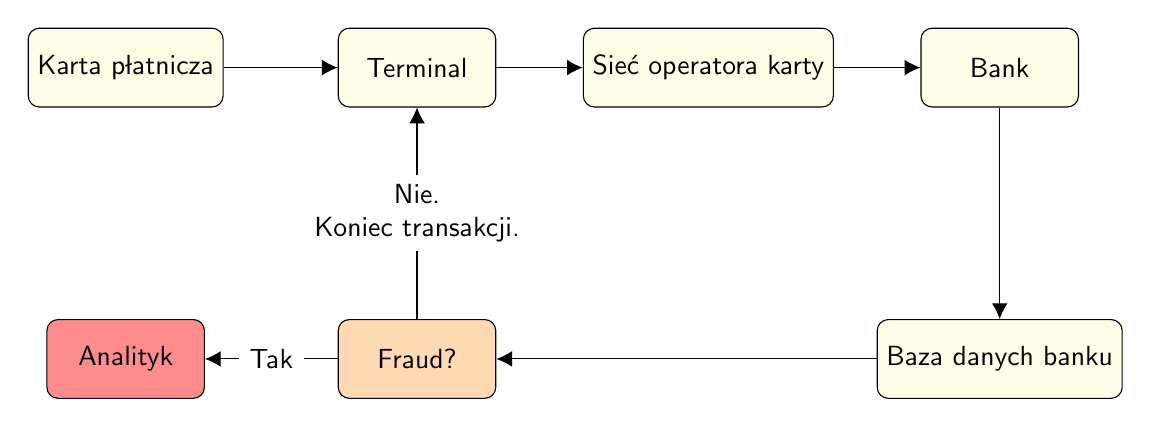
\begin{tikzpicture}[node distance=3.7cm,
	every node/.style={fill=white, font=\sffamily}, align=center]
	% Specification of nodes (position, etc.)
	\node (card)         [base]                        {Karta płatnicza};
	\node (terminal)     [base, right of=card]         {Terminal};
	\node (network)      [base, right of=terminal]     {Sieć operatora karty};
	\node (bank)         [base, right of=network]      {Bank};
	\node (db)           [base, below of=bank]         {Baza danych banku};
	\node (fraud)        [fraud, below of=terminal]    {Fraud?};
	\node (analitic)     [analityk, left of=fraud]     {Analityk};
	
	\draw[->] (card) -- (terminal);
	\draw[->] (terminal) -- (network);
	\draw[->] (network) -- (bank);
	\draw[->] (bank) -- (db);
	\draw[->] (db) -- (fraud);
	\draw[->] (fraud) -- node[text width=0.6cm] {Tak}(analitic);
	\draw[->] (fraud) -- node[text width=4cm] {Nie. \\Koniec transakcji.} (terminal);
	\end{tikzpicture}
\end{document}